%This work is licensed under the Creative Commons License Attribution 4.0 International (CC-BY 4.0)
%https://creativecommons.org/licenses/by/4.0/legalcode
\documentclass[rgb]{standalone}
\usepackage{tkz-euclide}
\usepackage{amsmath}
\definecolor{myorange}{hsb}{0.0833, 1, 0.8}
\definecolor{mygreen}{hsb}{0.3333, 1, 0.8}
\definecolor{myblue}{hsb}{0.5833, 1, 0.8}
\definecolor{mymagenta}{hsb}{0.8333, 1, 0.8}
\begin{document}
	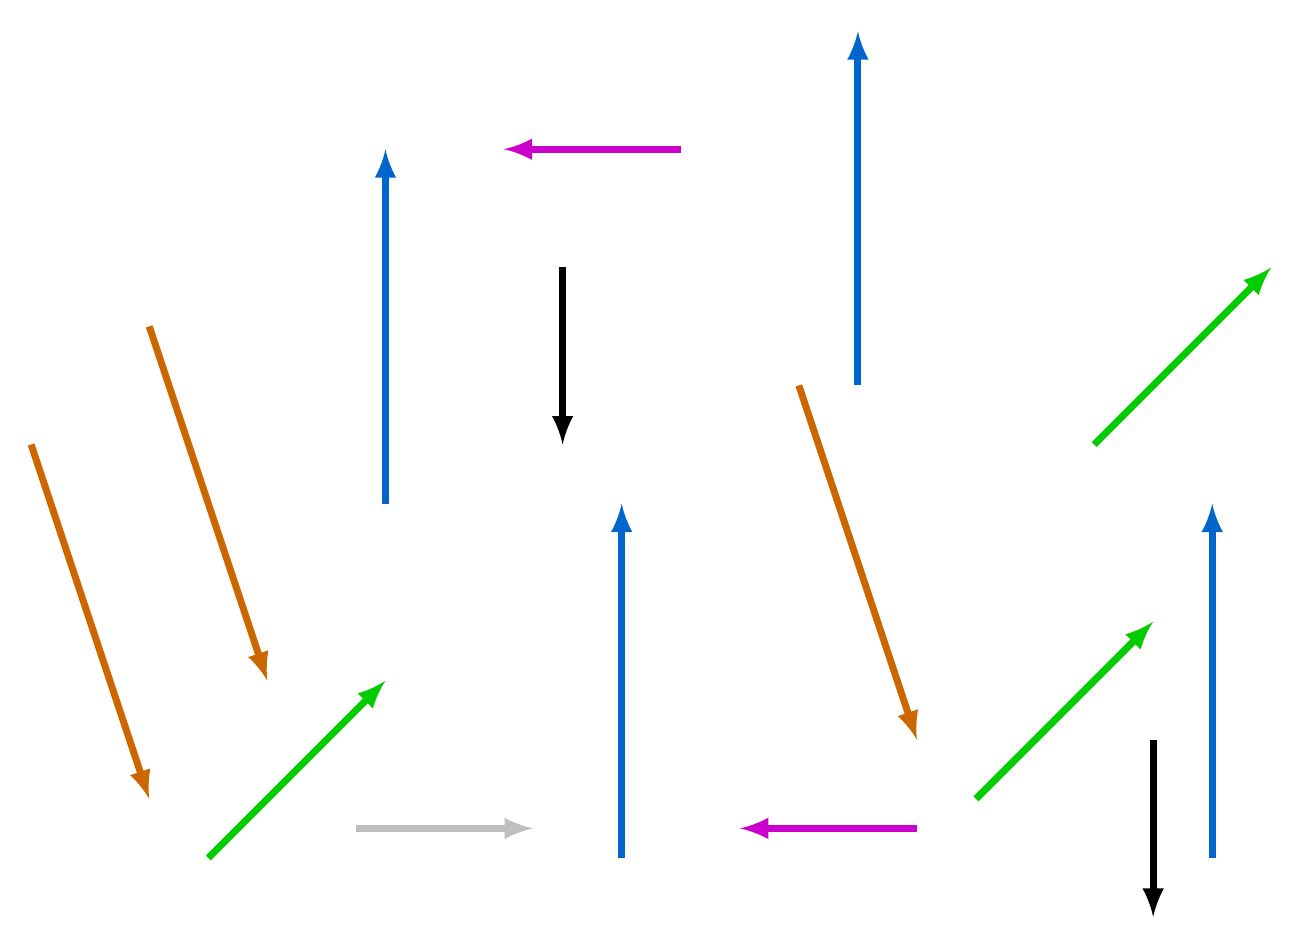
\begin{tikzpicture}[scale=1.5, font=\Large]
		\draw[line width=2.5pt,myblue,-latex] (0,0) -- (0,3);
		\draw[line width=2.5pt,myblue,-latex] (2,-3) -- (2,0);
		\draw[line width=2.5pt,myblue,-latex] (4,1) -- (4,4);
		\draw[line width=2.5pt,myblue,-latex] (7,-3) -- (7,0);
		\draw[line width=2.5pt,myorange,-latex] (-2,1.5) -- (-1,-1.5);
		\draw[line width=2.5pt,myorange,-latex] (-3,0.5) -- (-2,-2.5);
		\draw[line width=2.5pt,myorange,-latex] (3.5,1) -- (4.5,-2);
		\draw[line width=2.5pt,mygreen,-latex] (-1.5,-3) -- (0,-1.5);
		\draw[line width=2.5pt,mygreen,-latex] (5,-2.5) -- (6.5,-1);
		\draw[line width=2.5pt,mygreen,-latex] (6,0.5) -- (7.5,2);
		\draw[line width=2.5pt,mymagenta,-latex] (4.5,-2.75) -- (3,-2.75);
		\draw[line width=2.5pt,mymagenta,-latex] (2.5,3) -- (1,3);
		\draw[line width=2.5pt,lightgray,-latex] (-0.25,-2.75) -- (1.25,-2.75);
		\draw[line width=2.5pt,-latex] (1.5,2) -- (1.5,0.5);
		\draw[line width=2.5pt,-latex] (6.5,-2) -- (6.5,-3.5);
	\end{tikzpicture}
\end{document}